%% LyX 2.3.6 created this file.  For more info, see http://www.lyx.org/.
%% Do not edit unless you really know what you are doing.
\documentclass{article}
\usepackage[T1]{fontenc}
\usepackage[latin9]{inputenc}
\usepackage{geometry}
\geometry{verbose,tmargin=2cm,bmargin=2cm,lmargin=2cm,rmargin=2cm}
\usepackage{color}
\usepackage[spanish]{babel}
\addto\shorthandsspanish{\spanishdeactivate{~<>}}

\usepackage{textcomp}
\usepackage{url}
\usepackage{graphicx}
\usepackage[unicode=true,pdfusetitle,
 bookmarks=true,bookmarksnumbered=false,bookmarksopen=false,
 breaklinks=true,pdfborder={0 0 1},backref=false,colorlinks=true]
 {hyperref}

\makeatletter
%%%%%%%%%%%%%%%%%%%%%%%%%%%%%% User specified LaTeX commands.
\usepackage{charter}

\makeatother

\begin{document}
\title{Taller Docking Molecular con Autodock4 y SwissDock}
\author{Basado en el taller de Carlos Eduardo Bonilla}
\maketitle

\section{Objetivo}

Realizar el acomplamiento molecular de una prote�na y un ligando usando dos herramientas: Autodock tools y SwissDock. La primera se descarga e instala localmente mientras que la segunda se realiza el proceso en un servidor WEB.

\section{Moleculas}
\begin{description}
\item [{Prote�na:}] BCL-XL es una de las principales prote�nas que estimulan la supervivencia celular mediante la inhibici�n de la apoptosis al unirse e inhibir a prote�nas pro-apopt�ticas (Bax, Bak y posiblemente Bok) o a prote�nas BH3(1).
\item [{Ligando:}] La geniste�na, un qu�mico producido de forma natural presente en la soya, ha atra�do el inter�s cient�fico por sus posibles beneficios en la prevenci�n del c�ncer y enfermedad card�aca. La geniste�na es un tipo de qu�mico llamado fitoestr�geno - una sustancia similar al estr�geno presente en algunas plantas. Hay dos tipos principales de fitoestr�genos: isoflavonas y lignanos. La soya es la fuente m�s abundante de isoflavonas, con la geniste�na como la isoflavona m�s abundante en la soya. El tr�bol rojo tambi�n es una buena fuente de geniste�na (https://www.wnyurology.com/content.aspx?chunkiid=125001).
\end{description}

\section{Procedimiento}

\subsection{Instalaci�n software}
\begin{enumerate}
\item Descargar e instalar Autodock tools
\item Descargar e instalar Software Chimera.
\end{enumerate}

\subsection{Configurar carpeta de trabajo}
\begin{enumerate}
\item Crear una carpeta en su equipo donde van a guardarse las mol�culas y los resultados de la pr�ctica.
\item Configurar esta carpeta en preferencias de Autodock: Men� \textbf{File} \textrightarrow{} \textbf{Preferences}, se ajusta el Startup Directory con la ruta de su carpeta de trabaja y se selecciona \textquotedblleft Set\textquotedblright .
\end{enumerate}

\subsection{Descargar mol�culas }

Todos los resultados guardarlos en la carpeta de trabajo
\begin{enumerate}
\item Descargar estructura de la prote�na BCL-XL (PDB Id: 1lxl) desde el Protein Data Bank, en formato PDB. 
\begin{center}
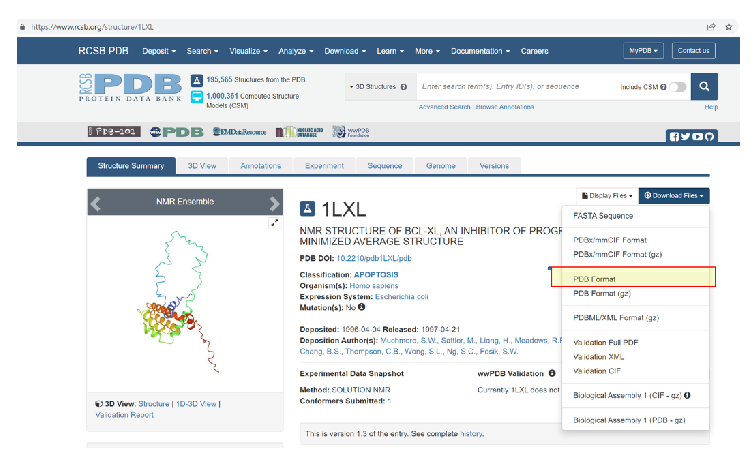
\includegraphics[scale=0.7]{images/PDB}
\par\end{center}
\item Descargar la estructura de ligando: \href{https://pubchem.ncbi.nlm.nih.gov/compound/Genistein}{geniste�na} (genistein) desde Pubchem (\url{https://pubchem.ncbi.nlm.nih.gov/compound/Genistein}), estructura 3D, formato SDF.
\begin{center}
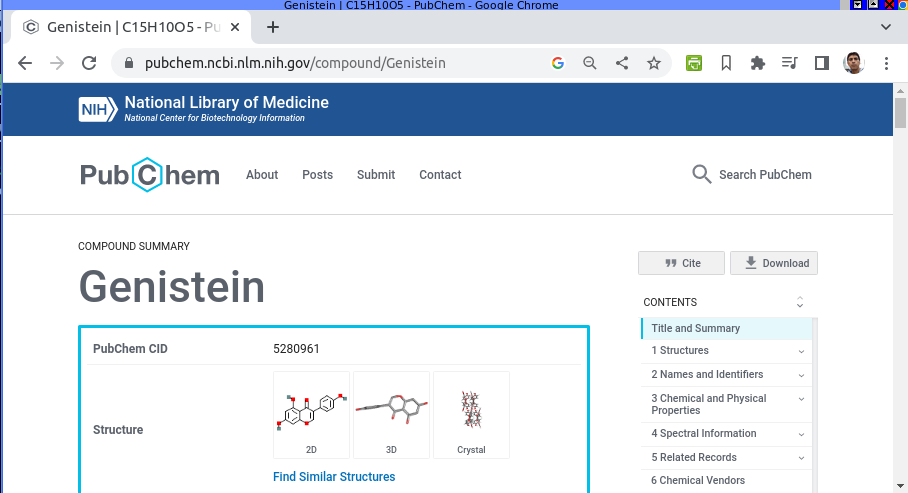
\includegraphics[scale=0.4]{images/pubchem-genistein}
\par\end{center}
\item Convertir archivo SDF de genisteina a formato mol2 utilizando el servidor de OpenBabel (\url{http://www.cheminfo.org/Chemistry/Cheminformatics/FormatConverter/index.html})
\begin{center}
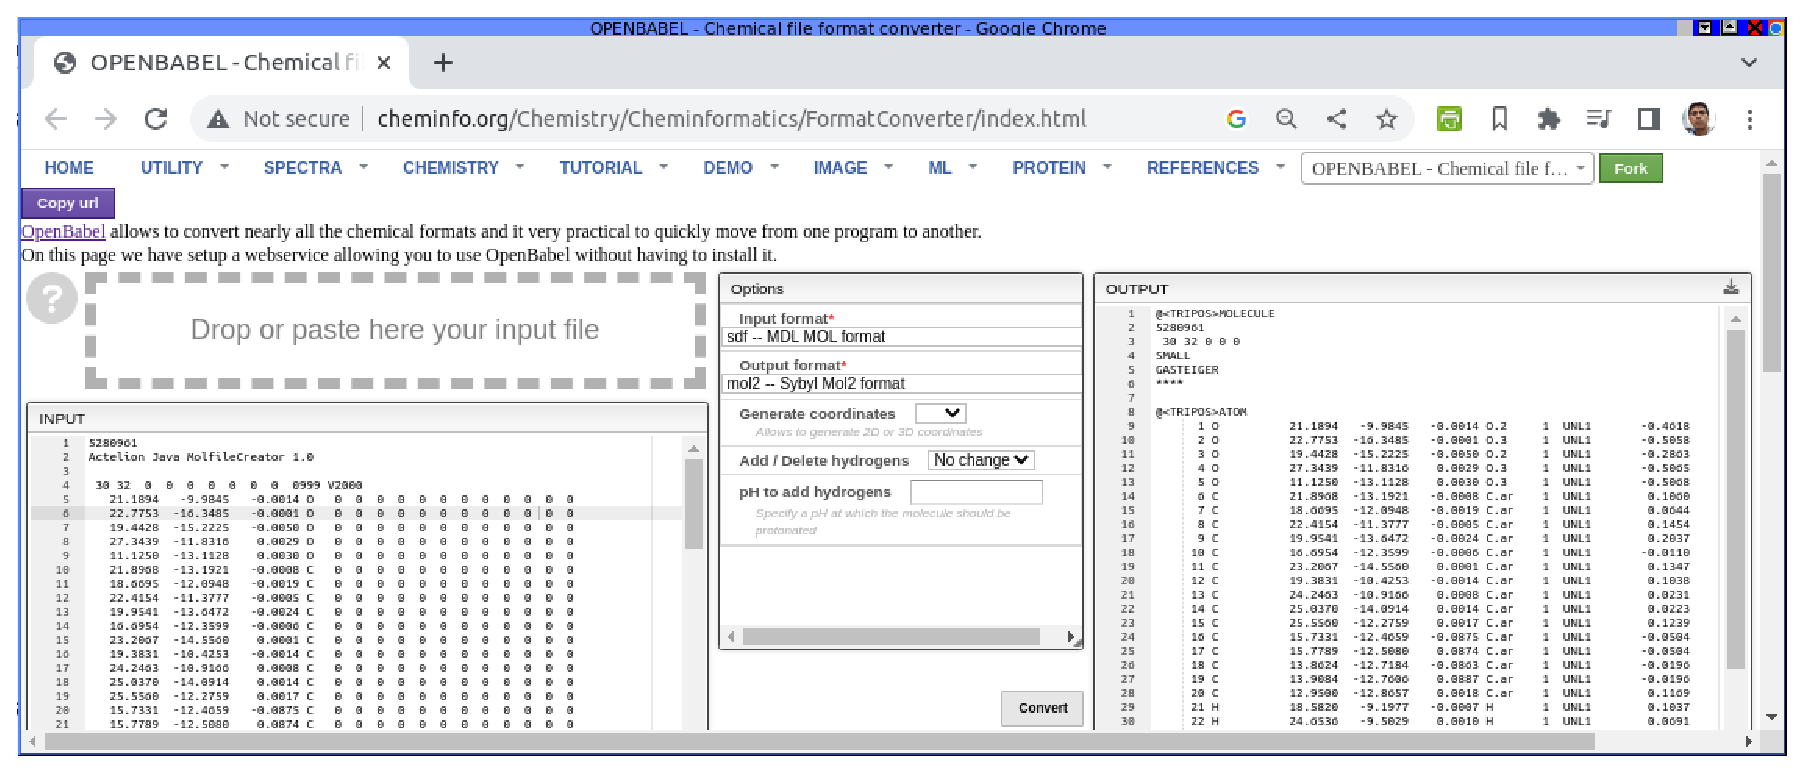
\includegraphics[scale=0.5]{images/openbabel-converter}
\par\end{center}
\end{enumerate}

\subsection{Cargar mol�culas a Autodock Tools}
\begin{enumerate}
\item Se carga ahora el archivo de la prote�na 1lxl.pdb: Men� \textbf{File} \textrightarrow{} \textbf{Read Molecule}. 
\begin{center}
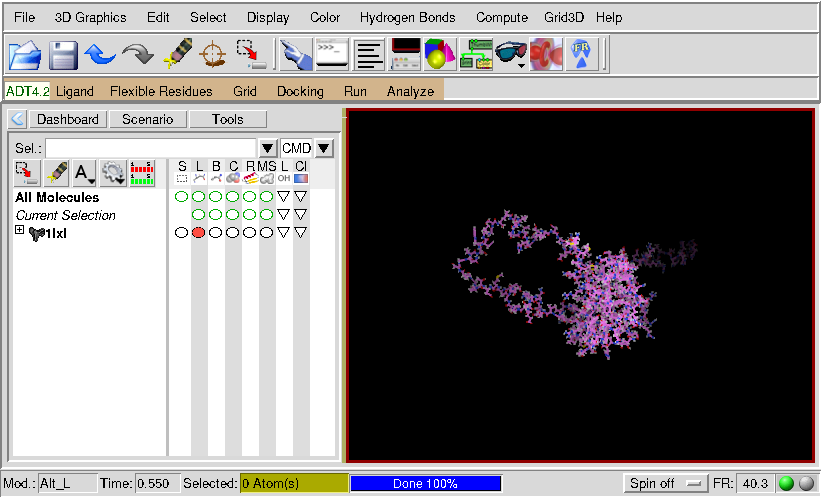
\includegraphics[scale=0.5]{images/Protein-load}
\par\end{center}
\item Cambiar la representaci�n gr�fica de la mol�cula de ''Lineas (Lines)'' a ''Cintas (Ribons)'', de-seleccione \textbf{''L'' }y seleccione \textbf{''R''}
\begin{center}
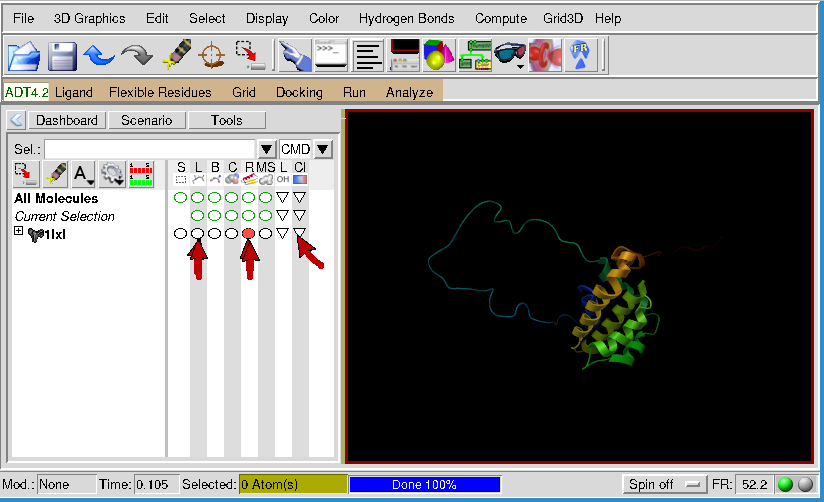
\includegraphics[scale=0.5]{images/Protein-representation2}
\par\end{center}
\item Preparar la prote�na: 
\begin{itemize}
\item En \textbf{Men� Edit}, se adicionan H+ polares (para a�adir cargas), se da OK. 
\item Luego se da click a Merge Non Polar. 
\item Y se adicionan cargas de Kollman para la prote�na. Las cargas de Kollman a�adidas son de -22.328
\begin{center}
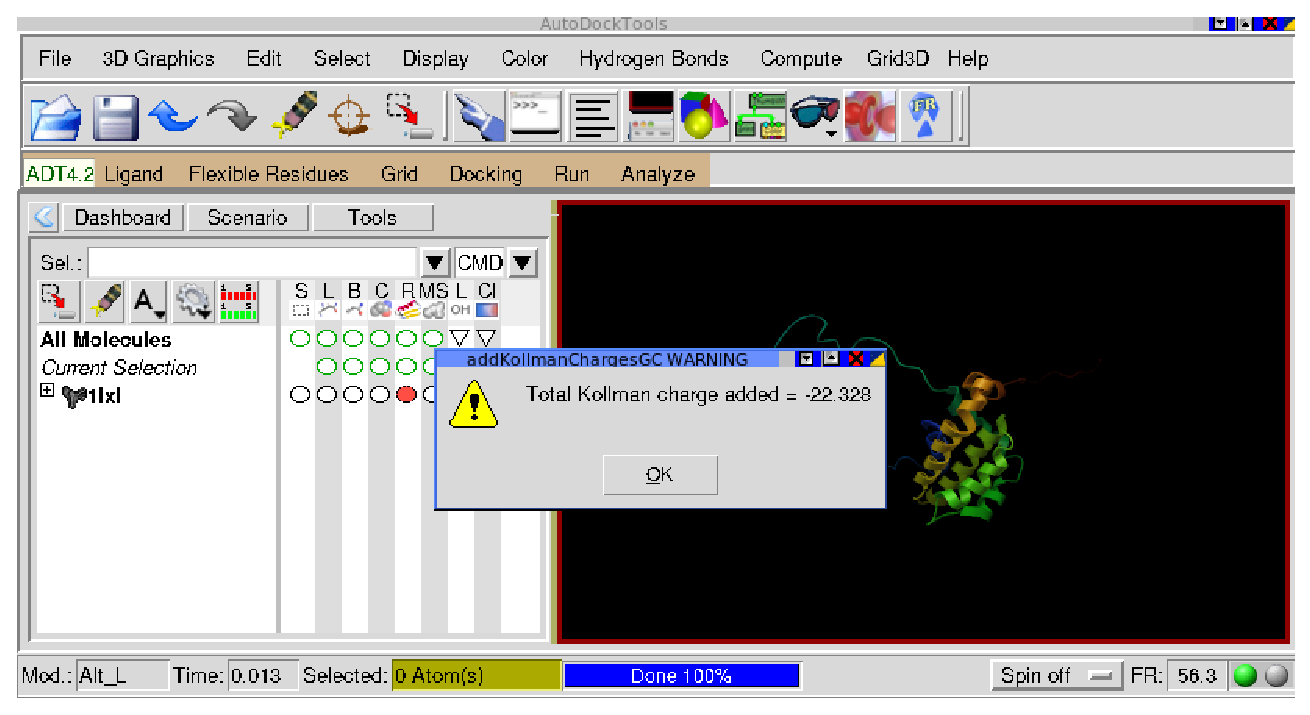
\includegraphics[scale=0.5]{images/Protein-charges}
\par\end{center}
\end{itemize}
\item Guardar los cambios de la mol�cula en formata PDBQ: Men� File , 
\item seleccionamos Save y luego Write PDB, se selecciona Sort Nodes (verificar direcci�n de guardado). Sobreesecribir
\end{enumerate}

\end{document}
